% ****** Start of file apssamp.tex ******
%
%   This file is part of the APS files in the REVTeX 4 distribution.
%   Version 4.0 of REVTeX, August 2001
%
%   Copyright (c) 2001 The American Physical Society.
%
%   See the REVTeX 4 README file for restrictions and more information.
%
% TeX'ing this file requires that you have AMS-LaTeX 2.0 installed
% as well as the rest of the prerequisites for REVTeX 4.0
%
% See the REVTeX 4 README file
% It also requires running BibTeX. The commands are as follows:
%
%  1)  latex apssamp.tex
%  2)  bibtex apssamp
%  3)  latex apssamp.tex
%  4)  latex apssamp.tex
%
\documentclass[prb,aps,twocolumn,preprintnumbers,amsmath,amssymb]{revtex4}
%\documentclass[preprint,showpacs,preprintnumbers,amsmath,amssymb]{revtex4}

% Some other (several out of many) possibilities
%\documentclass[preprint,aps]{revtex4}
%\documentclass[preprint,aps,draft]{revtex4}
%\documentclass[prb,twocolumn,showpacs,preprintnumbers,amsmath,amssymb]{revtex4}% Physical Review B

\usepackage{graphicx}% Include figure files
\usepackage{dcolumn}% Align table columns on decimal point
\usepackage{bm}% bold math
\usepackage[utf8]{inputenc}
\usepackage{url}
\newcolumntype{P}[1]{>{\centering\arraybackslash}p{#1}}
\newcolumntype{M}[1]{>{\centering\arraybackslash}m{#1}}
%\nofiles

\begin{document}

\title{Osciloscopio}% Force line breaks with \\

\author{Alejandro Hernández A.}%
 \email{a.hernandez105@uniandes.edu.co}
\author{Daniel Sánchez M.}%
 \email{d.sanches462@uniandes.edu.co}
\affiliation{%
Departamento de Física\\ Universidad de los Andes, Bogotá, Colombia.\\
}%


\date{3 de septiembre de 2015}% It is always \today, today,
             %  but any date may be explicitly specified

\begin{abstract}
Este informe presenta los datos obtenidos al medir voltaje y corriente para configuraciones solicitadas de circuitos RC y RLC. Para el circuito RC, se determinó el tiempo característico de carga y descarga de un condensador $C = 470 \mu F$, y se otuvieron los siguientes datos: $\tau_{exp} = (0.0534 \pm 0.025) s$ con error porcentual $E\% = 13.61 \%$ para $R = 100 \Omega$ y $\tau_{exp} = (0.0463 \pm 0.025) s$ con error porcentual $E\% = 75.82 \%$. Para el circuito RLC, determinó la frecuencia natural del sistema y el parámetro de resistencia y los datos obtenidos fueron los siguientes: $f_{0} = $ con error porcentual $E\% = \%$ y $\gamma = $ con error porcentual $E\% = \%$. 
\\

%\smallskip
\noindent \textbf{Conceptos clave:} Circuito RC, circuito RLC, oscilador amortiguado.
\end{abstract}
                             
\maketitle

\section{Introducción.}

Las resistencias, condensadores e inductancias son algunos de los elementos electrónicos de dos terminales más usados en diversos dispositivos tegnológicos de la actualidad. Y dado a que la implementación de los circuitos que usan estos elementos es relativamente simple, las características experimentales de estos elementos pueden ser estudiadas rigurosamente, ya sea con corriente directa DC o con corriente alterna AC.\\

En esta práctica nos interesan los circuitos RC y RLC, ambos en serie, cuyas principales características se presentan a continuación.


El circuito a usar se muestra en la figura\footnote{Imagen obtenida de https://www.flickr.com/photos/mitope\\ncourseware/3365787038\\} \ref{fig: RC}.

\begin{figure}[h!]
	\centering
	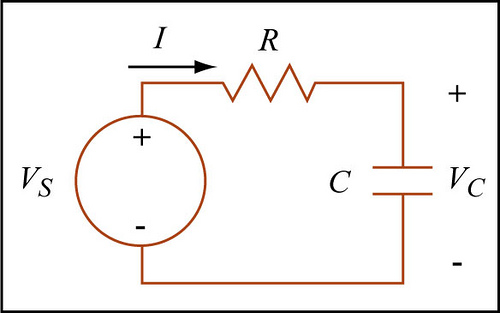
\includegraphics[width=0.4\textwidth]{RC}
	\caption{ Circuito RC en serie. }
	\label{fig: RC}
\end{figure} 

Para el proceso de carga del condensador, el voltaje a través de la resistencia viene dado por \eqref{VRC}.

\begin{equation}
\label{VRC}
V_{r} = V_{f}e^{-\frac{t}{RC}}
\end{equation}

Donde $V_{f}$ es el voltaje de la fuente (voltaje final del condensador).\\

Para el proceso de descarga el voltaje de la resistencia está dado por \eqref{RC}.

\begin{equation}
\label{RC}
V_{r} = -V_{0}e^{-\frac{t}{RC}}
\end{equation}

Donde $V_{0}$ representa el voltaje inicial del condensador.\\

En las ecuaciones anteriores la constante $\tau = RC$ tiene unidades de tiempo y corresponde al tiempo característico de carga o descarga del condensador de acuerdo a la situación de interés. Para el proceso de carga. Dicha constante es interpretada como el tiempo que tarda en cargarse (o descargarse) el condensador a un $67\%$ de su carga máxima.\\

Ahora bien, el circuito RLC a usar se muestra en la figura \footnote{Imagen obtenida de http://helios.augustana.edu/~dr/102/lectures/25.html\\} \ref{fig: RLC}.

\begin{figure}[h!]
	\centering
	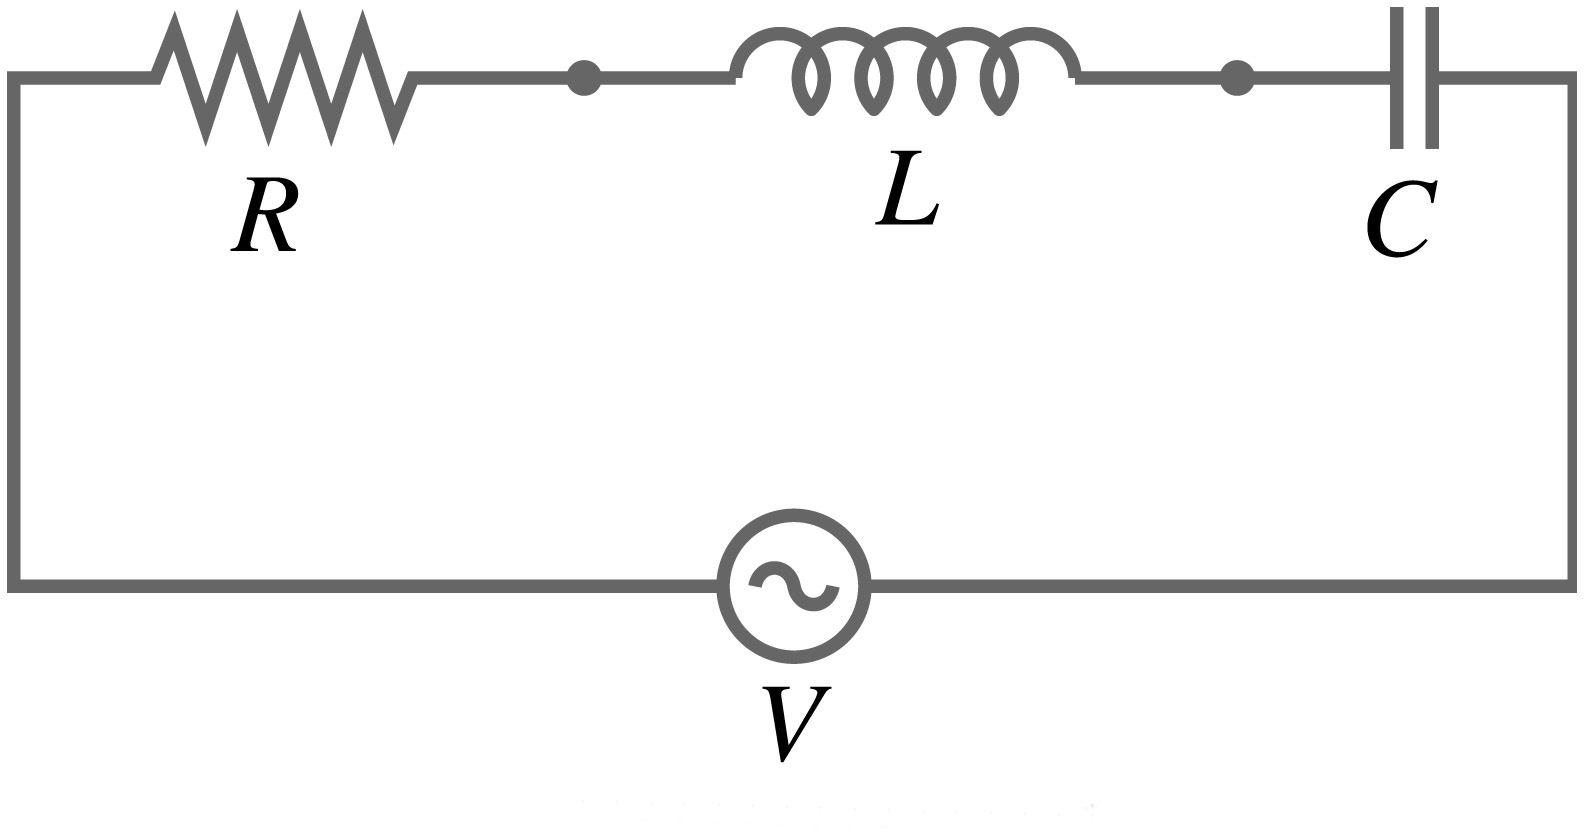
\includegraphics[width=0.4\textwidth]{RLC}
	\caption{Circuito RLC en serie}
	\label{fig: RLC}
\end{figure}

Este circuito es caracterizado por la ecuación \eqref{diff}.

\begin{equation}
\label{diff}
\frac{d^2 q}{d t^2} + \frac{R}{L}\frac{d q}{d t} + \frac{1}{LC}q = V(t)
\end{equation}

Donde $V(t)$ es el voltaje de la fuente, $\gamma = \frac{R}{L}$ es el factor análogo a la fricción en sistemas mecánicos que da cuenta de la disipación de energía en la resistencia, y $\omega_{0}^2 = \frac{1}{LC}$ es la frecuencia natural del sistema.\\

Suponiendo $V = \frac{V_{0}}{L} e^{i\omega t}$, el sistema está forzado y $\omega$ es la frecuencia de forzamiento y los parámetros $\gamma$ y $\omega_{0}$ determinan la resonancia del sistema con respecto al forzamiento  y determinan la existencia o no de soluciones oscilatorias cuando $\omega = 0$. Para dicha dependencia temporal del voltaje, la solución no homogénea\footnotemark[1] de la ecuación \eqref{diff} tiene la forma $q(t) = A(\omega) e^{i \omega t}$, con la amplitud dada por la ecuación \eqref{amplitud}.

\begin{equation}
\label{amplitud}
A(\omega) = \frac{V_{0}}{L}\frac{1}{\sqrt{(\omega^2 - \omega_{0}^2)^2+(\gamma \omega)^2}}
\end{equation}

Y la frecuencia de resonancia (frecuencia en la que la amplitud es máxima) está dada por la ecuación \eqref{resonancia}.

\begin{equation}
\label{resonancia}
\omega_{res} = \sqrt{\omega_{0}^2 - \frac{\gamma^2}{4}}
\end{equation}

De igual manera, el andho de la curva de resonancia está dado por:

\begin{equation}
\label{ancho}
\Delta \omega = \gamma = \frac{R}{L}
\end{equation}

Allende de lo anterior, es preciso hablar de las figuras de Lissajous, ya que serán mencionadas en secciones posteriores de este informe. Las figuras de Lissajous\footnotemark[2] son gráficas de un sistema con ecuaciones paramétricas dadas por:

\begin{equation}
\label{lissa}
\begin{split}
x &= A_{x}\sin(\omega_{x}t + \delta)\\
y &= A_{y}\sin(\omega_{y}t)
\end{split}
\end{equation}

Cabe mencionar que las condición para poder obtener figuras de Lissajous cerradas es que las frecuencias de las dos ondas superpuestas sean conmensurables, es decir, que sean números racionales. La visualización de estas curvas en un osciloscopio permiten verificar experimentalmente las cualidades teóricas de las superposición de en x y y de ondas producidas por un generador de señales.

\section{Montaje experimental}

Los instrumentos usados durante la práctica de laboratorio fueron un osciloscopio, dos generadores de señales, y diversos elementos electrónicos de dos terminales tales como resistencias, inductancias y condensadores.\\

\begin{figure}[h!]
	\centering
	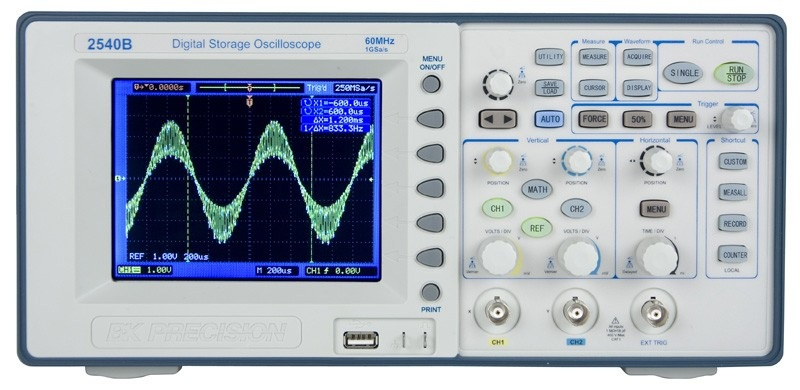
\includegraphics[width=0.4\textwidth]{osci}
	\caption{Osciloscopio usado para tomar de datos.}
	\label{fig: osci}
\end{figure}

\begin{figure}[h!]
	\centering
	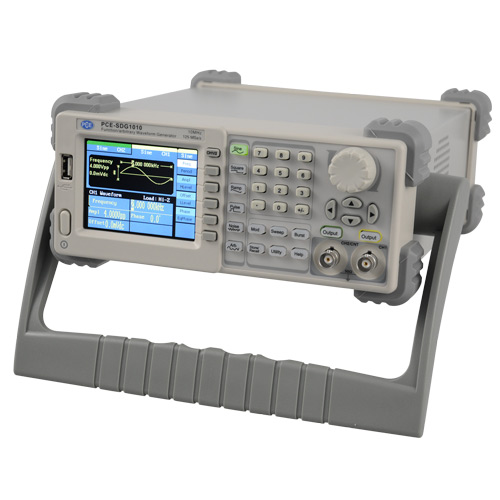
\includegraphics[width=0.4\textwidth,height=0.25\textheight]{generador}
	\caption{Generador de señales usado durante el laboratorio.}
	\label{fig: genr}
\end{figure}

El ocsilador y los generadores de señales se muestran en las figuras \footnote{Imágenes obtenidas de http://www.datuopinion.com/generador-de-senales} \ref{fig: osci} y \ref{fig: genr}.\\

En ensable de los circuitos mostrados en las figuras \ref{fig: RC} y \ref{fig: RLC} se hizo mediante cables proporcionados en el laboratorio, y las mediciones se realizaron con la ayuda de una sonda directamente conectada al osciloscopio que tenía caimanes en sus extremos.\\

En lo que respecta al circuito RC, para realizar las mediciones se usó una onda cuadrada de $5\ Hz$ con una amplitud de $5\ V$, una resistencia de $R = (470 \pm 1)\Omega$ y un condensador de capacitancia $C = (470 \pm 1)\mu F$. Se tomaron datos del voltaje de la resistencia.\\

Por su parte, para el circuito RLC se hicieron dos manipulaciones: en la primera se usó una onda sinusoidal de frecuencia $10\ Hz$ y de amplitud $5\ V$, un condensador de $C = (47 \pm 1)nF$ y una inductancia de $L = (2 \pm 1)mH$. Se tomaron datos del voltaje del condensador y se trató de determinar tanto la curva de resonancia como la frecuencia natural del sistema.\\

Para visualizar las figuras de Lissajous, se conectaron ambos generadores directamente al osciloscopio, cada uno de generando una onda sinusoidal de amplitud $5\ V$, y se observó la superposción de dichas ondas en el plano $xy$.

\section{Resultados y análisis}

Para el proceso de carga y descarga de un condensador de $C = 470 \mu F$ se usaron dos resistencias distintas ($R = 100 \Omega$ y $R = 470 \Omega$) en un circuito RC. Los datos obtenidos se muestran en las figuras \ref{fig: carga111}, \ref{fig: carga222} para la carga, y en las figuras \ref{fig: carga11}, \ref{fig: carga22} para la descarga.

\begin{figure}[h!]
	\centering
	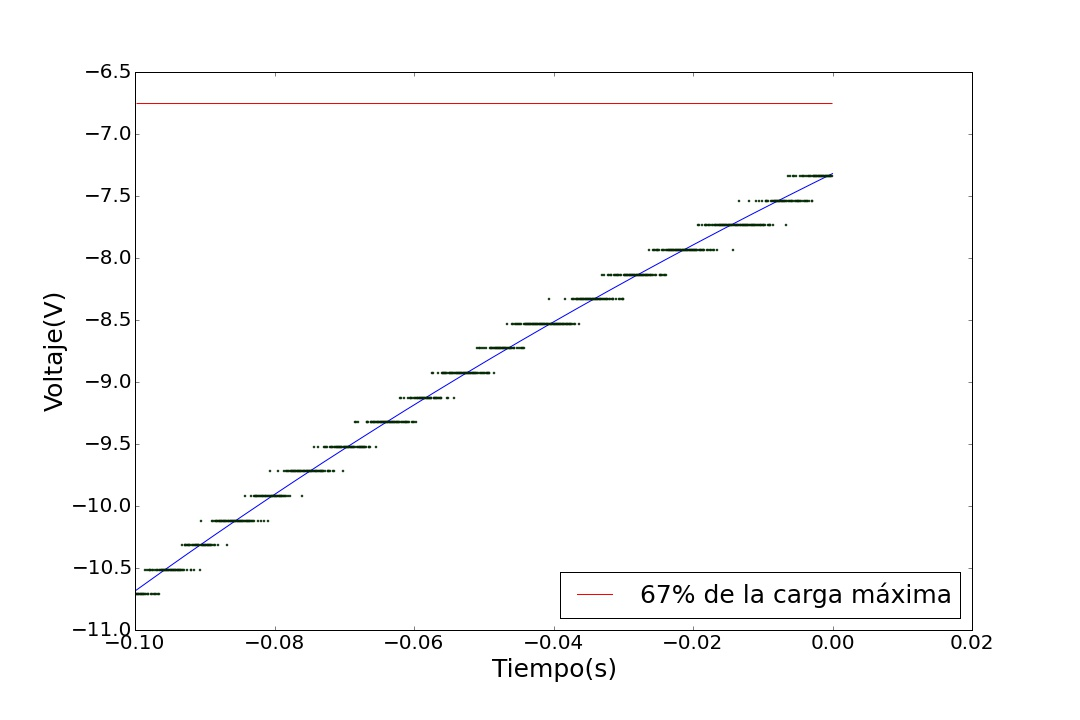
\includegraphics[width=0.5\textwidth,height=0.25\textheight]{carga111}
	\caption{Carga del condesador para los parámetros mencionados previamene de $R = 470 \Omega$ y $C = 470 \mu F$.}
	\label{fig: carga111}
\end{figure}

\begin{figure}[h!]
	\centering
	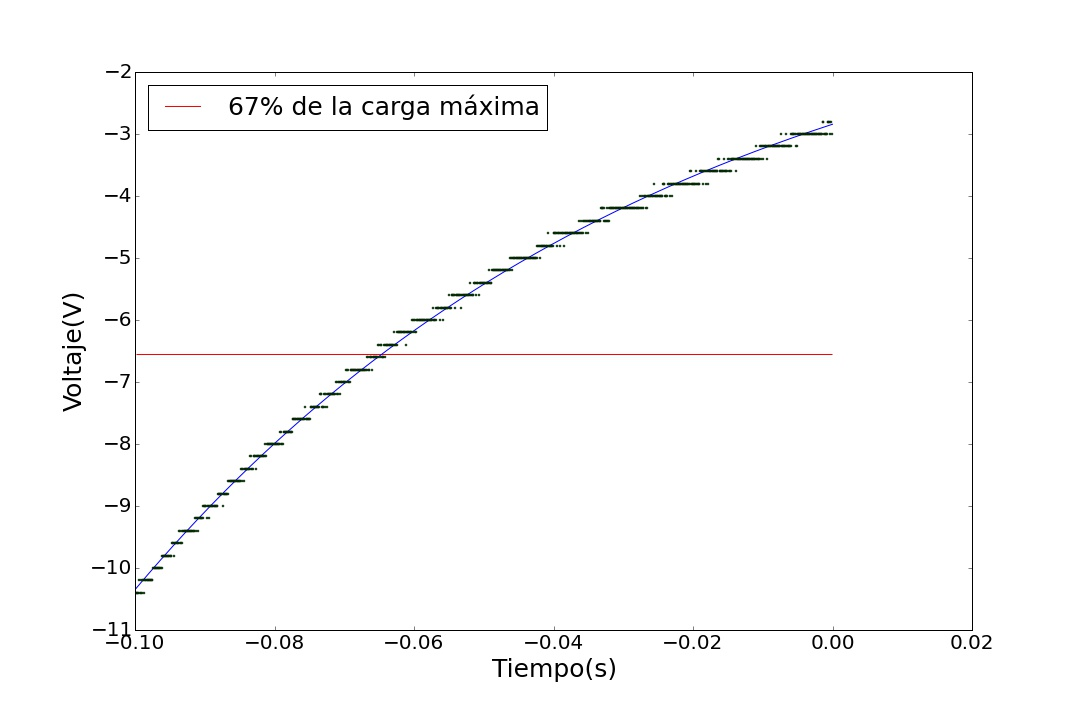
\includegraphics[width=0.5\textwidth,height=0.25\textheight]{carga222}
	\caption{Carga del condesador para los parámetros mencionados previamene de $R = 100 \Omega$ y $C = 470 \mu F$.}
	\label{fig: carga222}
\end{figure}

\begin{figure}[h!]
	\centering
	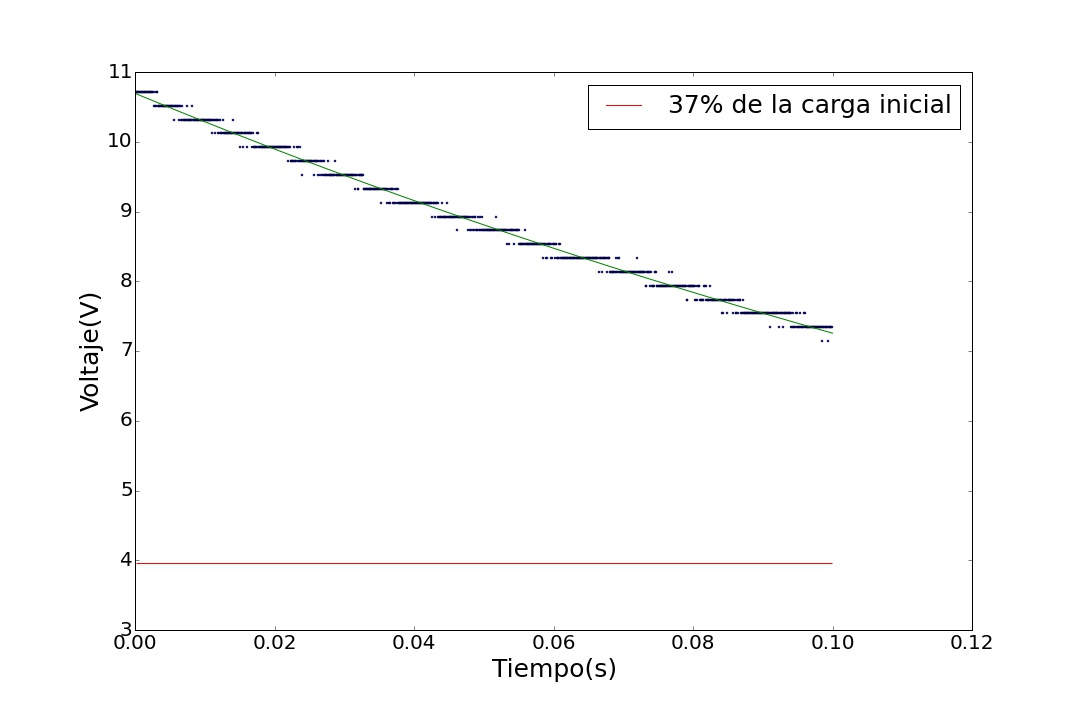
\includegraphics[width=0.5\textwidth,height=0.25\textheight]{carga11}
	\caption{Descarga del condesador para los parámetros mencionados previamene de $R = 470 \Omega$ y $C = 470 \mu F$.}
	\label{fig: carga11}
\end{figure}

\begin{figure}[h!]
	\centering
	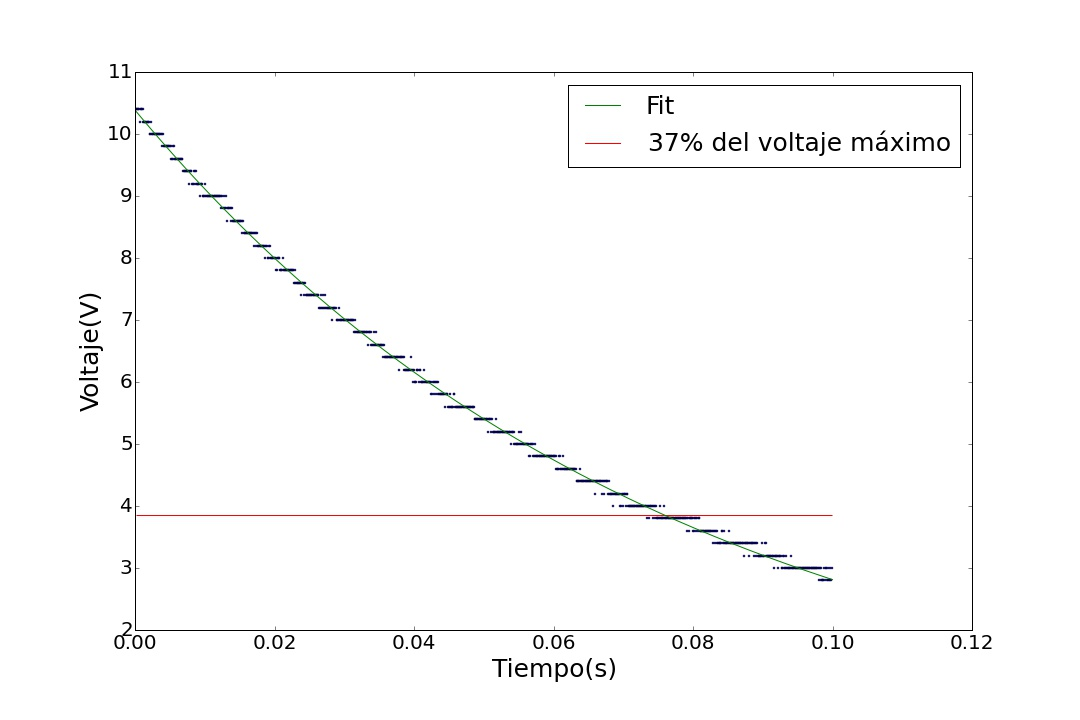
\includegraphics[width=0.5\textwidth,height=0.25\textheight]{carga22}
	\caption{Descarga del condesador para los parámetros mencionados previamene de $R = 100 \Omega$ y $C = 470 \mu F$.}
	\label{fig: carga22}
\end{figure}
\
\\
Los datos de tiempos característicos para las fases de carga y descarga se muestran en la tabla \ref{Tabla 1}.

\begin{table}[h!]
	\caption{\label{Tabla 1}Tiempos característicos de carga y descarga.}
	\begin{ruledtabular}
		\begin{tabular}{||M{2.5cm}|M{2.5cm}|M{2.5cm}||}
			Fase & $R (\Omega)$ & $\tau_{exp}$ (s)\\
			\hline
			Carga & 100 & 0.0534\\
			Descarga & 100 &  0.0534\\
			Carga & 470 & 0.0480\\
			Descarga & 470 & 0.0445\\
		\end{tabular}
	\end{ruledtabular}
\end{table}

Y promediando los datos tenemos que $\tau_{exp} = (0.0534 \pm 0.025) s$ para $R = 100 \Omega$ y $\tau_{exp} = (0.0463 \pm 0.025) s$ para $R = 470 \Omega$. Cabe aclarar que las incertidumbres etán dadas por la escala horizontal arrojada por el osciloscopio. Comparando dichos valores experimentales con los valores teóricos respectivos de $\tau_{teo} = 0.0470$ y $\tau_{teo} = 0.2209$, podemos ver que obtuvimos errores experimentales de $E\% = 	13.61 \%$ y $E\% = 75.82 \%$ respectivamente.\\

OJO - FALTA UN MAYOR ANÁLISIS\\

\begin{figure}[h!]
	\centering
	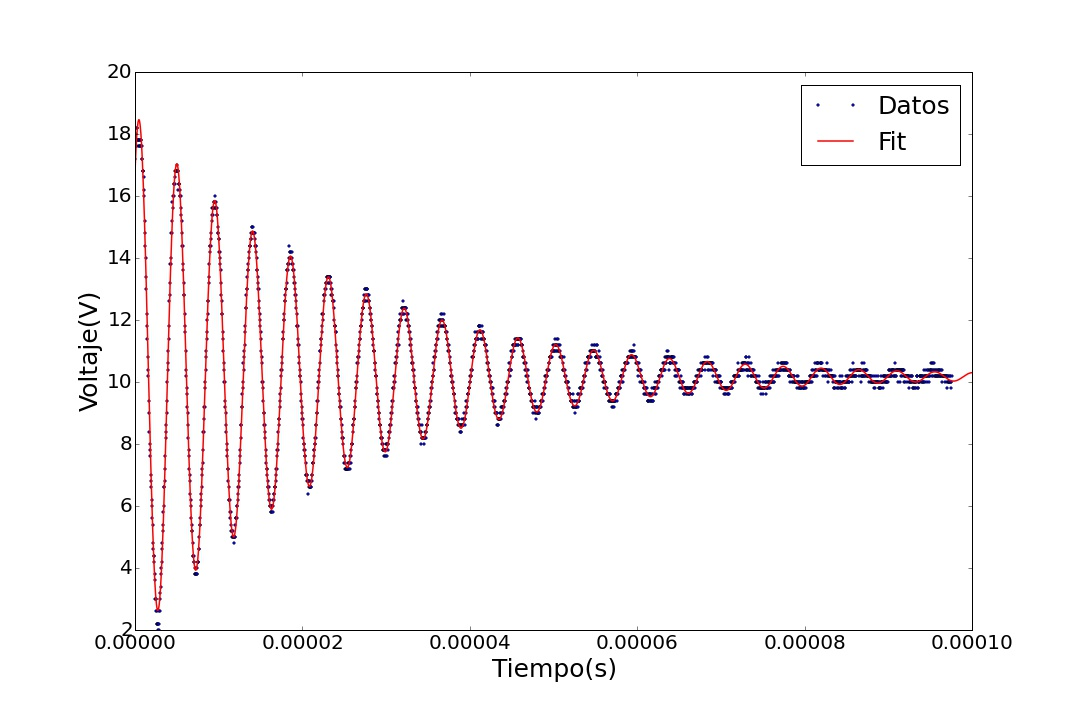
\includegraphics[width=0.5\textwidth,height=0.25\textheight]{amorti1}
	\caption{Potencial de un condensador en función del tiempo para un circuito RLC con $R = 1 kHz$, $L = 2 mH$ y $C = 51 pF$.}
	\label{fig: amorti1}
\end{figure}

En la figura \ref{fig: amorti1} se muestra el voltaje del condensador como función del tiempo para el circuito RLC en serie.\\

La función utilizada para hacer el fit no lineal fue la solución transiente del circuito RLC, a saber:

\begin{equation}
\label{transi}
V(t) = Ae^{- \gamma t}\sin(\omega ' t + \delta) + h
\end{equation}

Donde $h$ tan solo representa el voltaje alrededor del cual se realizan las oscilaciones en la figura \ref{fig: amorti1}. Dado esto, se obtuvieron los datos mostrados en la tabla \ref{Tabla 2}:

\begin{table}[h!]
	\caption{\label{Tabla 2}Parámetros óptimo otenidos del fit no lineal para $V(t)$ en presencia de una resistencia.}
	\begin{ruledtabular}
		\begin{tabular}{||M{2.5cm}|M{2.5cm}|M{2.5cm}||}
			Parámetro & Valor & Error estándar$^3$\\
			\hline
			A & 8.4571 V & 1.6487 $\cdot\ 10^{-2}$ V\\
			$\gamma$ & 4.1761 $\cdot\ 10^{4}\ 1/s$ & 1.1207 $\cdot\ 10^{2}\ 1/s$\\
			$\omega '$ & 1.3878 $\cdot\ 10^{6}\ 1/s$ &  1.1546 $\cdot\ 10^{2}\ 1/s$\\
			$\delta$ & 0.8965 rad & 1.9596 $\cdot\ 10^{-3}$ rad\\
			$h$ & 10.1719 V & 2.8124 $\cdot\ 10^{-3}$ V\\
		\end{tabular}
	\end{ruledtabular}
\end{table}

\begin{figure}[h!]
	\centering
	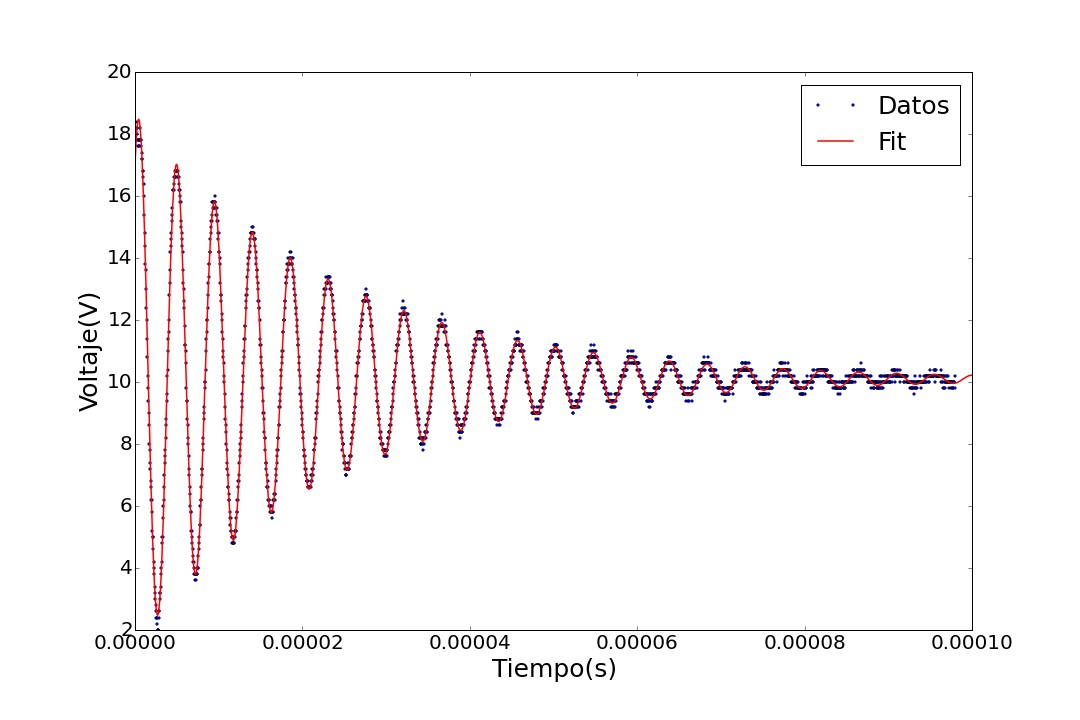
\includegraphics[width=0.5\textwidth,height=0.25\textheight]{amorti2}
	\caption{Potencial de un condensador en función del tiempo para un circuito LC con  $L = 2 mH$ y $C = 51 pF$.}
	\label{fig: amorti2}
\end{figure}

En la figura \ref{fig: amorti2} se muestra el voltaje del condensador como función del tiempo para el circuito LC en serie (ausencia de resistencia).\\

La función utilizada para hacer el fit no lineal fue nuevamente el voltaje dado por \eqref{transi} y se obtubieron los datos mostrados en la tabla \ref{Tabla 3}.\\\\\\\\\\\\\\\\

OJO - ANALIZAR LO QUE PASA CON LA RESISTENICIA, YO NO VEO NADA SIGNIFICATIVO.\\

\begin{table}[h!]
	\caption{\label{Tabla 3}Parámetros óptimo otenidos del fit no lineal para $V(t)$ en ausencia de una resistencia.}
	\begin{ruledtabular}
		\begin{tabular}{||M{2.5cm}|M{2.5cm}|M{2.5cm}||}
			Parámetro & Valor & Error estándar\\
			\hline
			A & 8.5367 V & 1.6487 $\cdot\ 10^{-2}$ V\\
			$\gamma$ & 4.2087 $\cdot\ 10^{4}\ 1/s$ & 1.1207 $\cdot\ 10^{2}\ 1/s$\\
			$\omega '$ & 1.3878 $\cdot\ 10^{6}\ 1/s$ &  1.1546 $\cdot\ 10^{2}\ 1/s$\\
			$\delta$ & 0.9411 rad & 1.9596 $\cdot\ 10^{-3}$ rad\\
			$h$ & 10.0950 V & 2.8124 $\cdot\ 10^{-3}$ V\\
		\end{tabular}
	\end{ruledtabular}
\end{table}

Con respecto a los datos para la curva de resonancia, cabe aclarar que apesar de que se trataron de obtener diversos datos con los cuales contruir la curva, no le obtuvieron datos razonables puesto que el máximo de la curva estaba muy alejado de lo previsto teóricamente. Sin embargo, los datos obtenidos se muestran en la figura \ref{fig: reso}.

\begin{figure}[h!]
	\centering
	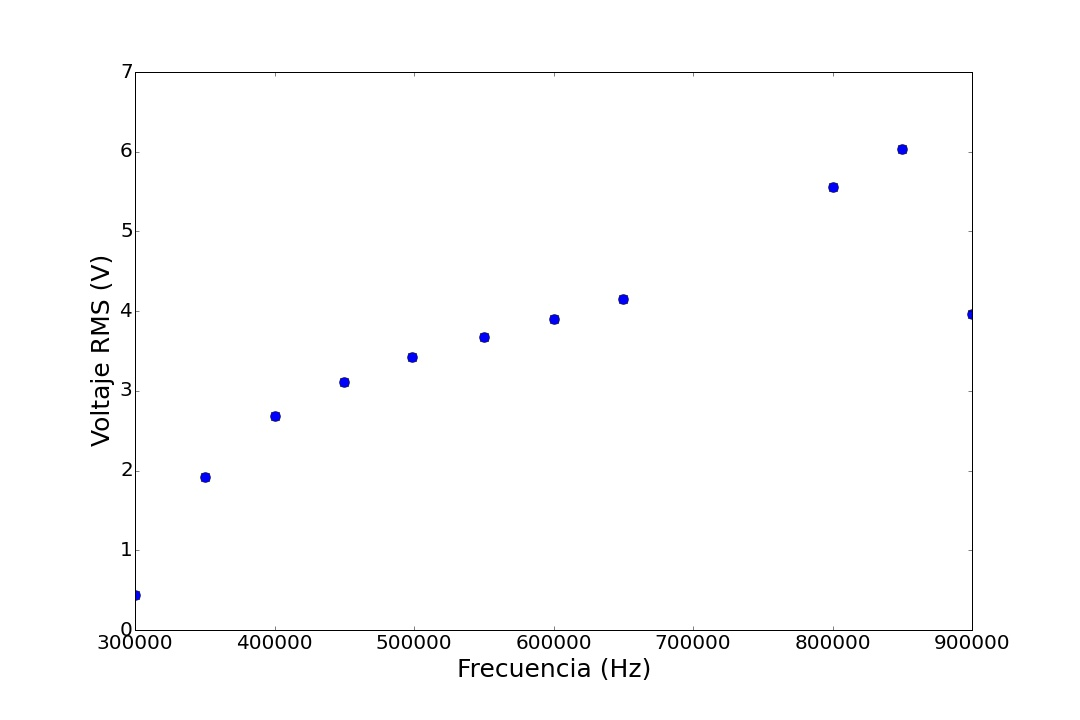
\includegraphics[width=0.5\textwidth,height=0.2\textheight]{reson}
	\caption{Datos obtenidos al tratar de medir la curva de resonancia para el circuito LC con $L = 2 mH$ y $C = 51 pF$.}
	\label{fig: reso}
\end{figure}

Claramente, no vale la pena tratar de analizar los datos a la luz de las ecuaciones \eqref{resonancia} y \eqref{ancho}, pero sí se puede decir que la potencial razón de la falla de la toma de datos radica en que, si bien se consideró que no había resistencia en el circuito de interés, todos los cables y elementos electrónicos de dos terminales presentan resistencias que, siendo pequeñas, no podían ser despreciadas para el cálculo teórico de la mencionada frecuencia de resonancia. \\

Además, cabe resaltar que no se usó el intrumento usual para realizar mediciones con el osciloscopio, es decir, la sonda especialmente diseñada para este fin, sino que se utilizó una sonda que tennía caimanes en sus extremos con el fin de facilitar la toma de datos. Se observó con este montaje y con los demás que esta sonda no era del todo confiable puesto que los datos cambiaban mucho dependiendo del agarre del caimán al istrumento al cual se le estaba midiendo el voltaje. Esta situación no pudo ser solucionada a pesar de que se cambió en repetidas veces la sonda usada para llevar a cabo las mediciones.\\

Finalmente, para la obtención de las figuras de Lissajous se fijó la misma amplitud para cada generador y se modificaron las frecuancias y los desfases de las ondas. El voltaje poco-a-pico registrado por el osciloscopio fue de 200 V y un ejemplo de las figuras observadas se muestra en \ref{fig: lissa}

\begin{figure}[h!]
	\centering
	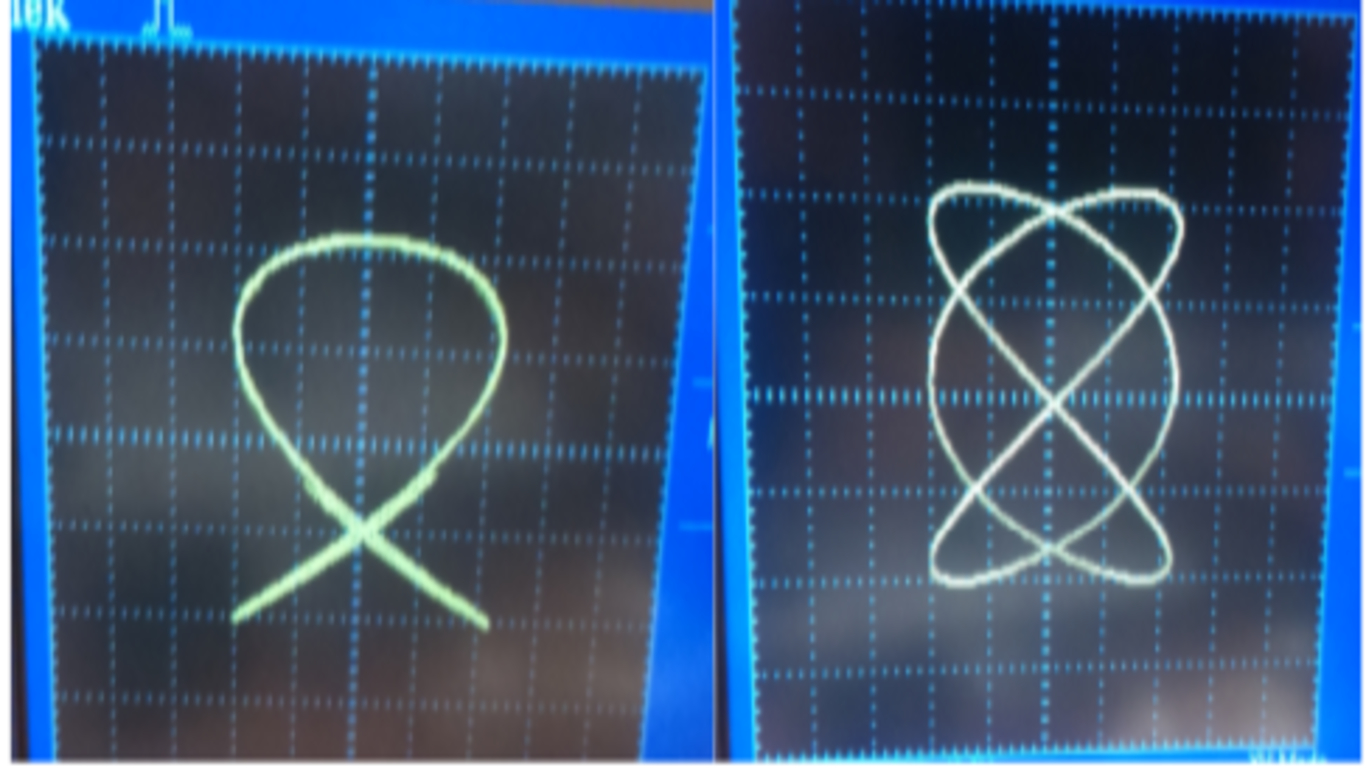
\includegraphics[width=0.5\textwidth,height=0.2\textheight]{lissa}
	\caption{Figuras de Lissajous para un a relación 1:3 de las frecuencias y desfases de 0 y  $\pi /2$.}
	\label{fig: lissa}
\end{figure}

Se observaron todas las proporciones y desfases ($\frac{\omega_{x}}{\omega_{y}} = 3, 2, \frac{3}{2}, \frac{3}{2}, \frac{4}{3}, \frac{6}{5},\ \delta = 0, \pi$) sugeridos por la guía pero no se referencian fotos dado a que el aspecto más relevante de esta parte de la práctica era verificar que las figuras de Lissajous son cerradas para frecuencias conmensurables, y dado a que, en efecto, se obtuvieron figuras cerradas para las relaciones sugeridas de las frecuencias, se verifica el comprtamiento experimental de la teoría correspondiente a la superposición de las ondas dadas por \eqref{lissa}.

\section{Conclusiones}

\begin{itemize}

	\item No se logró obtener la curva de resonancia para el circuito RC debido a potenciales errores en el cálculo teórico de la misma, así como a posibles factores de resistencia ignorados en los intrumentos utilizados para montar el circuito.
	
	\item Se logró verificar el comportamiento experimental de diversos elementos ondulatorios descritos teóricamente en el curso de Ondas Y fluidos, tales como circuitos RC, RLC, sistemas amortiguados y figuras de Lissajous.
		
	\item El buen uso de elementos de laboratorio tales como el osciloscopio, generadores de señales, y elementos electrónicos de dos terminales tales como resistencias, inductores y condensadores es fundamental a la hora de realizar mediciones experimentales de fenómenos ondulatorios.
	
	\item OJO.
	
\end{itemize}

\begin{thebibliography}{99}
\bibitem{french} A. P. French, {\it Vibrations and Waves}{The MIT Introductory Physics Series, USA, 1960}.\\
\bibitem{Tipler} Tipler, Paul A., \textit{Physics for scientists and engineers}. W.H. Freeman, 4 Edici\' on, 1999.\\
\bibitem{Taylor} Taylor, J.R., \textit{An Introduction to Error Analysis}. University Science Books, Sausalito, California. 2nd edition, 1982.\\
\end{thebibliography}

\end{document}
%
% ****** End of file apssamp.tex ******
